\documentclass[acmsmall,screen,nonacm]{acmart}

%% Course manuscript; ACM copyright block suppressed.
\settopmatter{printacmref=false}
\renewcommand\footnotetextcopyrightpermission[1]{}
\setcopyright{none}
\acmConference{}{}{}
\acmYear{2026}
\copyrightyear{2026}
\pagestyle{plain}

\usepackage{graphicx}
\usepackage{amsmath}
\usepackage{booktabs}
\usepackage{array}
\newcolumntype{L}[1]{>{\raggedright\arraybackslash}p{#1}}

\title{Effect of Citation-Count Features on Lower-Citation Recall in AI Literature Curation}

\author{Aditya Chaudhary}
\affiliation{%
  \institution{Indian Institute of Information Technology, Allahabad}
  \country{India}
}

\begin{abstract}
Scholarly search and screening tools often use citation counts as a ranking signal. This paper asks
whether adding an explicit citation-count feature to a transparent relevance ranker changes how many
relevant but rarely cited papers reach the top of a screening queue. Two Logistic Regression rankers that
differ only in a standardised $\log(1+\text{citations})$ feature are compared in two studies. Study 1, a
pilot, used a quota-stratified pool of 2,790 OpenAlex records on AI literature curation, screened by an AI
assistant with author review of the 458 relevant and boundary records. Only 7 of its 64 relevant records
were rarely cited, so the pre-registered dataset gate failed and its results are exploratory: in a
cross-fitted analysis the citation-blind ranker placed 7 of 7 lower-citation relevant records in the top
20\% of the queue against 3 of 7 for the citation-aware ranker (paired difference 0.57; 95\%
cluster-bootstrap interval 0.14 to 1.00). A blind re-screen of 200 AI-only labels found 3 missed relevant
records, all rarely cited; with them included the result was 9 of 10 against 3 of 10. Study 2 tested the
same hypothesis under a new pre-registration on the SYNERGY benchmark of systematic reviews with human
inclusion labels (20 reviews, 150,154 records, 2,745 relevant). The gate passed with 977 lower-citation
and 1,768 higher-citation relevant records. The citation-blind ranker retrieved 742 of 977 lower-citation
relevant records (0.759) against 691 of 977 (0.707) for the citation-aware ranker: a difference of 0.052
(interval 0.033 to 0.068), with no detectable change in overall recall. The citation feature moved recall
from rarely cited to highly cited relevant papers; the effect is confirmed but an order of magnitude
smaller than the pilot suggested, and it varied across reviews. Reserving half of the top-$K$ slots for
lower-citation records recovered 0.081 of lower-citation recall at a precision cost of 0.001.
\end{abstract}

\begin{CCSXML}
<ccs2012>
<concept>
<concept_id>10002951.10003317.10003338.10003341</concept_id>
<concept_desc>Information systems~Information retrieval</concept_desc>
<concept_significance>500</concept_significance>
</concept>
</ccs2012>
\end{CCSXML}
\ccsdesc[500]{Information systems~Information retrieval}

\keywords{citation bias, recall, literature screening, systematic review automation, feature ablation, OpenAlex, SYNERGY}

\begin{document}
\maketitle
\setlength{\emergencystretch}{2em}

\section{Introduction}
\label{sec:intro}

Many tools that help researchers find and screen literature rank records partly by how often they have
been cited. Google Scholar has been shown to weight citation counts heavily in its ranking
\cite{beel2009citation}, and scholarly recommenders are known to over-expose popular items
\cite{farber2023biases,klimashevskaia2024survey}. Citation counts are themselves shaped by cumulative
advantage \cite{merton1968matthew} and by factors unrelated to a study's content
\cite{duyx2017scientific,lund2025predictors}. If a ranker learns that relevant papers tend to be highly
cited, it may rank relevant but rarely cited papers lower, and in a prioritised screening workflow those
papers are the ones most likely to be left unread when screening stops \cite{callaghan2020stopping}.

Evaluations of screening tools usually report recall for a whole collection
\cite{przybyla2018prioritising,vandeschoot2021asreview,aigner2026comparing}. Whether that recall is
lower for less-cited papers is rarely measured: the author's earlier survey of recall bias in AI
literature curation \cite{chaudhary2026recall} found that evaluations of screening and citation-searching
tools report recall for whole collections and never split it by citation band or language, and named this
as an open gap. This study takes up that gap and isolates one mechanism: it trains two
otherwise identical rankers, one with and one without an explicit citation-count feature, and compares
how many relevant lower-citation records each places in the top $K$ of a held-out queue.

The paper reports two studies. Study 1 (Sections~\ref{sec:data}--\ref{sec:results}) is a pilot on a
small, carefully audited pool of AI literature-curation records; its pre-registered data gate failed, so
its results are exploratory. Study 2 (Section~\ref{sec:study2}) tests the hypothesis that the pilot
suggested, under a separate pre-registration written before its data were downloaded, on a large public
benchmark with human inclusion labels. Neither study estimates how any commercial search engine behaves,
and neither tests language effects.

\section{Research Questions}
\label{sec:rq}

\begin{description}
\item[RQ1 (primary).] In a fixed candidate pool, does adding a $\log(1+\text{citations})$ feature to a
TF--IDF Logistic Regression ranker change Recall@K for relevant lower-citation records? The contrast is
$\Delta_{\text{low}} = \text{Recall}_{\text{low}}@K(A) - \text{Recall}_{\text{low}}@K(B)$, where $A$ is
citation-blind and $B$ citation-aware; a positive value favours $A$.
\item[RQ2.] Does the citation feature change the gap between higher- and lower-citation recall?
\item[RQ3 (conditional).] Do English and non-English metadata-language records differ? This was to be
analysed only if publication languages were verified and each group had at least 20 relevant test
records.
\end{description}

The frozen protocol made no prediction about the direction of $\Delta_{\text{low}}$.

\section{Data}
\label{sec:data}

\subsection{Candidate pool}

The pool was collected from the OpenAlex API \cite{priem2022openalex} on 30 October 2026 (citation
snapshot date). Three kinds of route were used, each restricted to records with abstracts published
2015--2025: eight English keyword queries (for example \emph{automated literature screening},
\emph{scholarly information retrieval}, \emph{active learning title abstract screening}) and four OpenAlex
topic filters, each sampled at 20 records per publication year with OpenAlex's seeded random sampling;
and the incoming citers and outgoing references of five seed papers on screening, citation searching,
scholarly recommender bias and language bias in retrieval. No route was sorted by citation count. After
deduplication by OpenAlex identifier the pool held 2,790 records, with 247--262 records in each year.
The pool is a quota-stratified sample of query frames, not a census, so all recall values are relative to
it.

\subsection{Metadata audit}

Before screening, 27 records were withheld: 6 whole-issue records verified on publisher pages, 13
records with missing titles that could not be repaired from source, and 8 administrative records
(retraction flags, retraction notices, errata and a superseded version). Duplicate and version
relationships were reviewed manually and recorded in a \texttt{split\_group\_id}; one two-version group
was found. The OpenAlex language field is inferred from metadata and can be wrong
\cite{cespedes2025openalex}; it is called \emph{metadata language} here because no publication language
was verified.

\subsection{Relevance screening and label provenance}

Records were screened on title and abstract against Annotation Rubric v2. A record is relevant only if it
studies, develops or evaluates a computational or AI method whose target task is discovering, ranking,
recommending, screening or selecting scholarly literature. Reviews of AI in an application domain,
downstream extraction from study content, and bibliometric analyses are not relevant.

\textbf{Screening procedure and label provenance.} Screening ran in two stages. First, an AI assistant
(Claude, Anthropic) applied Rubric v2 to all 2,763 records, recording a label, a coded rationale and a
confidence level for each. A seeded random 20\% of its decisions (550 records, seed 20261030) was
re-screened by the same assistant without access to its first-pass labels: 549 of 550 agreed. Second, the
author reviewed every record that the first pass marked relevant or uncertain (72), every negative it had
examined closely (53), and every remaining negative containing curation-related terms (333), 458 records in
all, assigning their own label, rationale and confidence. Author and AI agreed on 443 of the 458 records
(Cohen's $\kappa = 0.88$). The author changed 15 decisions: one uncertain record became relevant, four
relevant and two uncertain records became not relevant, and eight became uncertain. Records the author
marked uncertain (9) are excluded from modelling. The other 2,305 records, which the first pass judged
clearly unrelated to scholarly-literature curation, were not individually reviewed by the author and keep
the AI label; their status is recorded as \texttt{ai\_provisional} in the data files.

Table~\ref{tab:screening} summarises the outcome. Of 2,754 decided records, 64 were relevant. They cover
machine-assisted screening, scholarly search and discovery systems, citation-based searching, paper
recommendation and review automation. Relevance was very unevenly distributed across routes: 46 relevant
records (72\%) were reached through citation neighbourhoods, which contributed only 145 decided records,
whereas the 1,740 keyword-route records contained 10 relevant records (0.6\%).

\begin{table}[t]
\caption{Screening outcome by retrieval route (final labels). Records reached by several routes are
counted in each.}
\label{tab:screening}
\small
\begin{tabular}{L{4.2cm}rrr}
\toprule
Route & Decided records & Relevant & Relevant (\%) \\
\midrule
Keyword search (8 queries) & 1,740 & 10 & 0.6 \\
Topic filter (4 topics) & 865 & 5 & 0.6 \\
Citation neighbourhood (5 seeds) & 145 & 46 & 31.7 \\
Seed papers & 5 & 4 & 80.0 \\
\midrule
All decided records & 2,754 & 64 & 2.3 \\
\bottomrule
\end{tabular}
\end{table}

\section{Methods}
\label{sec:methods}

\subsection{Rankers}

Both conditions use the same scikit-learn pipeline \cite{pedregosa2011scikit}: TF--IDF features of title
and abstract (unigrams and bigrams, minimum document frequency 2, sublinear term frequency) plus
standardised publication year, and Logistic Regression ($C = 1$, balanced class weights, liblinear
solver, random state 20261030). Condition B adds one standardised feature,
$\log(1 + \text{citations})$, with scaling fitted on training data only. Nothing else differs. Each
condition ranks the test records by predicted probability, breaking ties by OpenAlex identifier.

\subsection{Citation groups and metrics}

Citations are adjusted for exposure time as a citation rate, citations divided by
$\max(1, 2026 - \text{year} + 1)$. Records at or below the pool median rate (0.408 citations per year)
form the lower-citation group. The group definition is not a field-normalised impact measure. The
primary metric is lower-citation Recall@K with $K = \lceil 0.20 N_{\text{test}} \rceil$: the share of
relevant lower-citation test records ranked in the top $K$. Overall Recall@K, Precision@K and
higher-citation Recall@K are secondary; $K$ at 10\% and 30\% are pre-specified sensitivity analyses.

\subsection{Frozen design and dataset gate}

The frozen protocol uses five-fold \texttt{StratifiedGroupKFold} (seed 20261030) with fold 0 as test,
fold 1 as validation and folds 2--4 as training, so that version groups never cross partitions. Before
any model is fitted, the test fold must contain at least 20 relevant lower-citation and 20 relevant
higher-citation records. The paired difference is bootstrapped by resampling \texttt{split\_group\_id}
clusters (2,000 replicates, seed 20261031). The protocol's success rule requires $\Delta_{\text{low}} > 0$,
a bootstrap lower bound above 0 and a Precision@K loss of no more than 0.05 for condition A.

\subsection{Amendment A3: exploratory analyses}

Amendment A3 was recorded before any model was fitted, once screening showed that the gate could not
pass. It specifies: (i) the gate is reported as failed; (ii) the frozen single-split comparison is still
run, labelled exploratory; and (iii) a cross-fitted analysis uses each of the same five folds once as the
test fold, training on the other four. Recall@K is computed within each fold and pooled across folds
(relevant records ranked in the top $K$ of their fold, divided by all relevant records), and the paired
difference is bootstrapped by resampling clusters within folds. After the frozen exploratory run returned
a degenerate result (Section~\ref{sec:frozen}), a reporting guard was added that marks the primary
estimate as not estimable when fewer than 10 relevant lower-citation test records are present; this is
disclosed in the amendment addendum and changes no estimate.

\section{Results}
\label{sec:results}

\subsection{Dataset gate}

The gate failed. Relevant records were concentrated among highly cited works: their median citation
count was 38, against 2 for non-relevant records, and only 7 of the 64 fell in the lower-citation group.
The frozen test fold contained 13 relevant records, 1 in the lower-citation group and 12 in the
higher-citation group. Training data contained 38 relevant records, of which 5 were lower-citation.

\subsection{Frozen single split (exploratory)}
\label{sec:frozen}

The citation-blind ranker placed all 13 relevant test records in the top $K = 111$ of 551 records; the
citation-aware ranker placed 10, missing two higher-citation records and the single lower-citation record, so $\Delta_{\text{low}} = 1$ and the bootstrap interval was the degenerate $[1, 1]$.
With one record in the denominator this comparison carries no information beyond that single case and is
reported as not estimable. Precision@K was 0.117 for condition A and 0.090 for condition B.

\subsection{Cross-fitted analysis (exploratory)}

Table~\ref{tab:crossfit} and Figure~\ref{fig:recall} give pooled results over the five folds. The
citation-blind ranker placed all 7 lower-citation relevant records in the top 20\% of their test folds;
the citation-aware ranker placed 3. The paired difference in lower-citation Recall@20\% was 0.57 (95\%
cluster-bootstrap interval 0.14 to 1.00). Higher-citation recall changed less (0.982 against 0.947;
difference 0.035, interval 0.000 to 0.088). Overall recall fell from 0.984 to 0.891 (difference 0.094,
interval 0.019 to 0.167), and Precision@20\% fell slightly, from 0.114 to 0.103. The citation feature
therefore did not buy any gain in this pool; it lowered both overall and lower-citation recall.

\begin{table}[t]
\caption{Cross-fitted pooled results (five folds, final labels, exploratory). Counts are relevant records in
the top $K$ of their fold over relevant records.}
\label{tab:crossfit}
\small
\begin{tabular}{lrrrr}
\toprule
 & \multicolumn{2}{c}{Citation-blind (A)} & \multicolumn{2}{c}{Citation-aware (B)} \\
\cmidrule(lr){2-3}\cmidrule(lr){4-5}
Group, $K$ & hits & recall & hits & recall \\
\midrule
Lower-citation, 20\% & 7/7 & 1.000 & 3/7 & 0.429 \\
Higher-citation, 20\% & 56/57 & 0.982 & 54/57 & 0.947 \\
All relevant, 20\% & 63/64 & 0.984 & 57/64 & 0.891 \\
\addlinespace
Lower-citation, 10\% & 7/7 & 1.000 & 1/7 & 0.143 \\
Lower-citation, 30\% & 7/7 & 1.000 & 6/7 & 0.857 \\
All relevant, 10\% & 63/64 & 0.984 & 52/64 & 0.812 \\
\bottomrule
\end{tabular}
\end{table}

\begin{figure}[t]
\centering
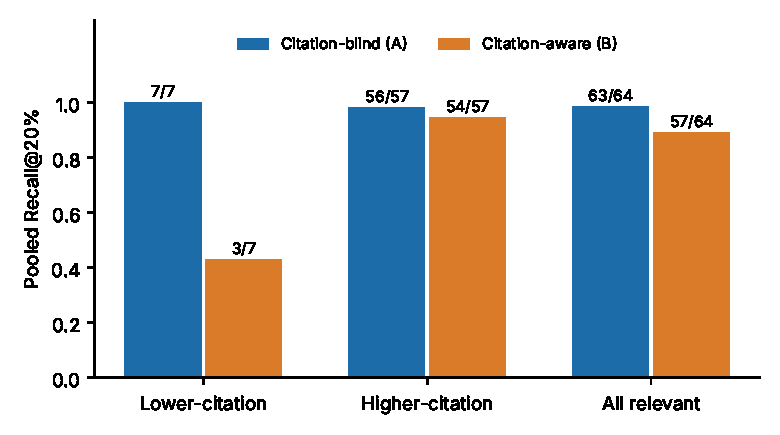
\includegraphics[width=0.68\linewidth]{fig_recall_by_group.pdf}
\caption{Pooled Recall@20\% by citation group in the cross-fitted analysis. Labels give relevant records
in the top $K$ over relevant records in the group.}
\label{fig:recall}
\end{figure}

The pre-specified sensitivity cutoffs show the same direction (Table~\ref{tab:crossfit}): at 10\% the
citation-aware ranker retrieved 1 of 7 lower-citation relevant records, and at 30\% it retrieved 6 of 7,
while the citation-blind ranker retrieved all 7 at every cutoff.

\subsection{Post-hoc reference rankers (not pre-registered)}

After the cross-fitted results were seen, two reference rankers were scored on the same folds from the
committed out-of-fold predictions, without refitting the two pre-registered rankers
(Table~\ref{tab:posthoc}). A \emph{citation-only} ranker, which orders each fold by
$\log(1+\text{citations})$ alone, retrieved none of the 7 lower-citation relevant records and 37 of 64
relevant records overall. A \emph{fair re-rank} kept the citation-aware scores but reserved half of the
top-$K$ slots for the best-scoring lower-citation records (share fixed at 0.5, not tuned). It recovered all 7
lower-citation records (difference from citation-aware 0.57, interval 0.14 to 1.00) but not the overall
loss: its overall recall, 0.906, stayed below the citation-blind ranker's 0.984 (difference 0.078, interval
0.016 to 0.145). In this pool, removing the citation feature did better than correcting for it afterwards.
Both comparisons are post hoc and exploratory.

\begin{table}[t]
\caption{Post-hoc reference rankers on the same five folds, $K = 20\%$ (exploratory, not pre-registered).}
\label{tab:posthoc}
\small
\begin{tabular}{lrrr}
\toprule
Ranker & Lower-citation & All relevant & Precision@20\% \\
\midrule
Citation-blind (A) & 7/7 & 63/64 & 0.114 \\
Citation-aware (B) & 3/7 & 57/64 & 0.103 \\
Citation-only & 0/7 & 37/64 & 0.067 \\
Fair re-rank (B, 50\% reserved) & 7/7 & 58/64 & 0.105 \\
\bottomrule
\end{tabular}
\end{table}

\subsection{Blind spot-check of AI-only labels (Amendment A4)}
\label{sec:spotcheck}

To measure the error in the 2,305 labels that the author had not reviewed, a simple random sample of 200
of them (seed 20261110, drawn and committed before review) was re-screened by the author under Rubric v2,
with the AI label and citation counts hidden. The author agreed with the AI on 190 of 200 records. Three
records the AI had called not relevant were judged relevant (1.5\%; exact 95\% interval 0.3\% to 4.3\%),
which scales to about 35 missed relevant records among the 2,305 (interval 7 to 100). Seven more had
no usable abstract and were marked uncertain. All three missed relevant records fell in the lower-citation
group: they are obscure, non-English or regional papers that the AI screener had treated as off-topic.

Correcting only the 200 sampled records (3 added as relevant, 7 excluded as uncertain) and re-running the
unchanged pipeline gave 67 relevant records, 10 of them lower-citation; the dataset gate still failed. In
the cross-fitted analysis the citation-blind ranker retrieved 9 of 10 lower-citation relevant records at
$K = 20\%$ and the citation-aware ranker 3 of 10 (paired difference 0.60; 95\% interval 0.33 to 1.00);
higher-citation recall was 56 of 57 for both, and overall recall was 0.970 against 0.881. The direction
and size of the effect are unchanged. The main results above use the labels frozen before this check;
both versions are in the repository.

\subsection{Error analysis}

Figure~\ref{fig:rankshift} shows where the seven lower-citation relevant records were ranked within their
test folds. All had between 0 and 3 citations. Under the citation-blind ranker they sat at ranks 1 to 40;
under the citation-aware ranker four moved below the cutoff, to ranks between 126 and 280, and the other
three fell from ranks 1--20 to ranks 10--93. Two were published in 2025 and two in 2024, so they have had
little time to be cited; others are older papers that never attracted citations, for example a 2015 article
on using full-text citation networks to improve keyword labelling. The seven records are spread across all
five folds (three in one fold, one in each of the others). Among higher-citation relevant records, an
Indonesian-language thesis-search system was missed by both rankers (ranks 514 and 384), and two records
with six citations each, a library discovery-tool evaluation and a search system for the COVID-19 research
collection, were retrieved by the citation-blind ranker (ranks 38 and 34) but not by the citation-aware
ranker (ranks 120 and 117).

\begin{figure}[t]
\centering
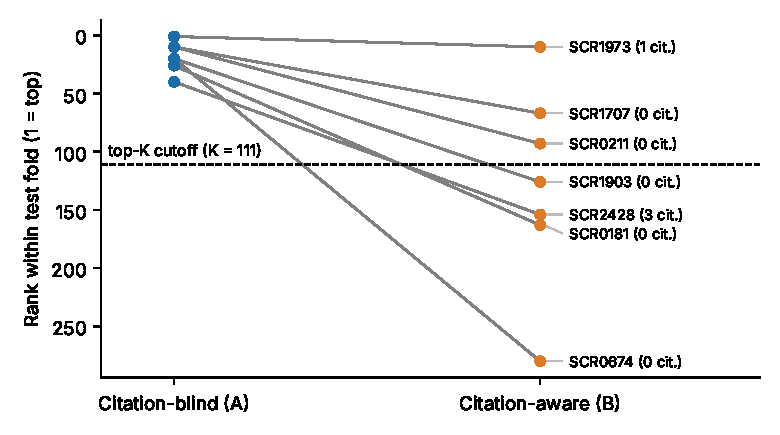
\includegraphics[width=0.68\linewidth]{fig_rank_shift_lower_citation.pdf}
\caption{Rank within test fold of the seven relevant lower-citation records under each ranker. Smaller
ranks are better; the dashed line marks the top-$K$ cutoff in a 551-record fold.}
\label{fig:rankshift}
\end{figure}

\subsection{Language}

Of the 64 relevant records, 61 had English metadata, and one each Spanish, Indonesian and Thai. No publication
language was verified. RQ3 cannot be addressed with these data.

\subsection{Resources}

Each ranker took about one second to fit and about 0.2 seconds to score a 551-record fold on a standard
CPU; the full cross-fitted analysis with 2,000 bootstrap replicates took about 30 seconds.

\section{Study 2: Pre-registered Confirmatory Test on SYNERGY}
\label{sec:study2}

\subsection{Rationale and pre-registration}

Study 1 pointed in one direction but could not confirm it. Study 2 therefore tested a directional
hypothesis on new data. The pre-registration was written by the author on 13 November 2026, before any
Study 2 data were downloaded, and fixed the following. \textbf{H1 (primary):} the citation-blind ranker
achieves higher lower-citation Recall@20\% than the citation-aware ranker. \textbf{H2:} reserving top-$K$
slots for lower-citation records recovers lower-citation recall relative to the citation-aware ranker at
a precision cost of at most 0.05. \textbf{H3 (descriptive):} a citation-only ranker shows how far ranking
by citations alone favours highly cited records. The gate required at least 50 relevant records in each
citation group, pooled over reviews and folds (Study 1 used 20). H1 is supported only if the gate passes,
the paired difference and the lower bound of its 95\% interval are above zero, and the citation-blind
ranker loses no more than 0.05 precision. The model, features, folds, seeds and $K$ rule are those of
Study 1; the reserved share (0.5) and precision limit were carried over unchanged.

\subsection{Data}

SYNERGY \cite{debruin2023synergy} contains 26 systematic reviews with 169,288 records and 2,834
inclusions decided by the original review teams; each record is linked to OpenAlex. Publication year and
citation count were available for 168,856 records. As pre-registered, reviews with fewer than 20
inclusions were dropped, leaving 20 reviews, 150,154 records and 2,745 relevant records (prevalence
1.8\%). Most reviews are in medicine and the health and behavioural sciences; two are in software engineering. No screening was done for this
study and no AI-assigned labels are used.

Each review is analysed separately, because relevance is defined by that review's own question. Within a
review, records are split into five grouped folds (records with the same normalised title share a
group), each fold is scored by rankers trained on the other four, and the citation groups are defined by
a median split of the age-adjusted citation rate within the review. Counts are pooled over folds and
reviews, and paired differences are bootstrapped by resampling title groups within review and fold
(2,000 replicates).

\subsection{Deviations recorded before any result}

Two changes were recorded before any model was fitted. First, the download tool's default had changed to
a larger collection (SYNERGY+); the original SYNERGY named in the pre-registration was selected
explicitly. Second, the plan to fetch citation counts live from OpenAlex failed twice on the provider's
rate limit after 90,100 records, so the citation counts and years stored in the SYNERGY release were used
instead, with the latest publication year in the data (2022) as the reference year for the age
adjustment. These counts are closer in time to the reviews than counts taken in 2026 would be.

\subsection{Results}

The gate passed: 977 relevant records were in the lower-citation group and 1,768 in the higher-citation
group. Table~\ref{tab:study2} gives the pooled results at $K = 20\%$. The citation-blind ranker retrieved
742 of 977 lower-citation relevant records (0.759) and the citation-aware ranker 691 (0.707), a paired
difference of 0.052 (95\% interval 0.033 to 0.068). Overall recall did not differ detectably (0.789
against 0.793; difference $-0.004$, interval $-0.015$ to 0.003), and precision was the same to three
decimals (difference $-0.0004$). All conditions of the success rule are met, so \textbf{H1 is supported}.
The difference had the same sign at $K = 10\%$ (571 against 538 of 977) and $K = 30\%$ (827 against 798).

\begin{table}[t]
\caption{Study 2, pooled over 20 SYNERGY reviews, $K = 20\%$ (confirmatory).}
\label{tab:study2}
\small
\begin{tabular}{lrrrr}
\toprule
Ranker & Lower-citation & Higher-citation & All relevant & Precision \\
\midrule
Citation-blind & 742/977 (0.759) & 1424/1768 (0.805) & 0.789 & 0.072 \\
Citation-aware & 691/977 (0.707) & 1486/1768 (0.840) & 0.793 & 0.072 \\
Citation-only & 0/977 (0.000) & 896/1768 (0.507) & 0.326 & 0.030 \\
Fair re-rank (50\% reserved) & 770/977 (0.788) & 1364/1768 (0.771) & 0.777 & 0.071 \\
\bottomrule
\end{tabular}
\end{table}

The citation feature did not lower recall overall; it moved it between groups. Higher-citation recall
rose from 0.805 to 0.840 with the feature (difference $-0.035$ for blind minus aware, interval $-0.048$
to $-0.026$; this contrast was not pre-registered and is descriptive). The gap between the two citation
groups was 0.046 for the citation-blind ranker and 0.133 for the citation-aware ranker.

\textbf{H2 is supported.} The fair re-rank retrieved 770 of 977 lower-citation relevant records, 0.081
more than the citation-aware ranker (interval 0.062 to 0.100), at a precision cost of 0.001; it lowered
overall recall by 0.016 (interval 0.006 to 0.027). For H3, the citation-only ranker retrieved none of the
lower-citation relevant records at $K = 20\%$. This is close to true by construction, since the
lower-citation group is defined by the quantity that ranker sorts on, and is reported only as a reference
point; its overall recall was 0.326.

\begin{figure}[t]
\centering
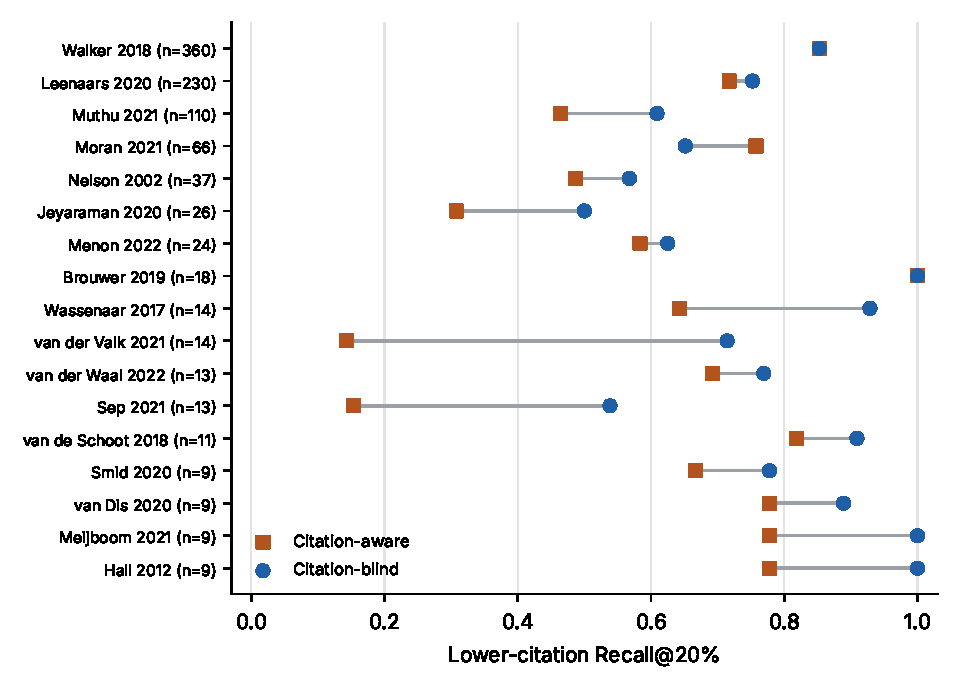
\includegraphics[width=0.74\linewidth]{fig_study2_per_review.pdf}
\caption{Study 2: lower-citation Recall@20\% in each review with at least five lower-citation relevant
records ($n$ = number of such records).}
\Description{Dot plot with one row per SYNERGY review, comparing lower-citation recall for the
citation-blind and citation-aware rankers. The citation-blind ranker is higher in most reviews, equal in
two, and lower in one.}
\label{fig:study2}
\end{figure}

\subsection{Consistency across reviews}

The pooled effect is not uniform (Figure~\ref{fig:study2}). Among the 19 reviews with at least one
lower-citation relevant record, the citation-blind ranker retrieved more of them in 14, the same number
in 4 and fewer in 1 (Moran 2021: 43 against 50 of 66). The largest review, Walker 2018, contributes 360
of the 977 lower-citation relevant records and showed no difference (307 against 307), which pulls the
pooled estimate down: without it the difference is 0.083, and without the two largest reviews 0.111
(post-hoc, descriptive). In the software-engineering review with enough records to show
(Hall 2012), the counts were 9 of 9 against 7 of 9. The effect therefore depends on the review, and the
pooled figure should be read as an average over reviews of very different size.

\section{Discussion}
\label{sec:discussion}

In Study 1, the cross-fitted result points the way the motivating concern predicts. When relevant records in the
training data are mostly highly cited, a citation feature becomes a proxy for relevance, and relevant
records that are rarely cited are pushed down the queue even when their text clearly matches the task. In
this pool the cost was not confined to the lower-citation group: overall recall also fell, because highly
cited but irrelevant records displaced relevant ones from the top $K$.

Three features of the data limit how far this can be taken. First, the comparison rests on seven records;
the within-fold bootstrap does not capture variation from model refitting or fold composition, so the
interval is likely too narrow. Second, the citation advantage of relevant records is largely an
artefact of collection. Seventy-two per cent of relevant records came from the citation neighbourhoods of
five seed papers, which are by construction connected to cited work; keyword routes with random sampling
returned mostly off-topic records. A pool built differently could show a very different citation profile
among relevant records, and the effect of the citation feature depends on that profile. Third, the records the author did not review keep AI labels, and the blind spot-check
(Section~\ref{sec:spotcheck}) shows this matters: an estimated 35 relevant records are missing among them,
and those found were all rarely cited. The AI screener's misses therefore fall on exactly the group this
study measures, so the true lower-citation group is probably larger than 7. The effect held when the three
found records were added, but a full review of the unreviewed records would be needed to settle it.

Study 1 alone therefore does not show that citation features harm lower-citation recall. It shows that
the measurement is feasible, that the direction is consistent with the concern, and that the denominators
needed for a confirmatory test are far larger than its pool provides.

Study 2 supplied those denominators and confirmed the direction: with 977 lower-citation relevant
records, removing the citation feature raised their Recall@20\% by 0.052. Two things changed relative to
the pilot. The effect is about a tenth of the pilot's point estimate, which is what a seven-record
estimate with an interval from 0.14 to 1.00 should lead one to expect; the pilot was right about the sign
and uninformative about the size. And overall recall did not fall. In Study 2 the citation feature
redistributed recall: highly cited relevant records gained about as much as rarely cited ones lost, so a
whole-collection recall figure would have shown nothing. That is the gap identified in the review that
motivated this work: an evaluation that reports only overall recall cannot see this trade-off.

For practice, the result suggests that a screening tool can drop a citation feature at no measurable
cost in overall recall or precision, and that where the feature is kept, a simple reserved-slot re-rank
recovers lower-citation recall for a small loss in overall recall. Both statements hold for a linear
ranker on these reviews and would need testing on other models.

\section{Threats to Validity}
\label{sec:threats}

\textbf{Construct validity.} Relevance is defined narrowly by Rubric v2; a broader definition would change
prevalence and the citation profile of relevant records. The citation group is a pool-median split of an
age-adjusted rate, not field-normalised impact.

\textbf{Internal validity.} The two rankers differ in one feature only, so differences between them are
attributable to that feature within this pool. Labels were assigned by an AI screener and, for the 458
boundary and relevant records, reviewed by the author, who knew the study's question; citation counts were
not shown in the screening sheets. A blind random spot-check of 200 unreviewed AI labels found 3 missed
relevant records (Section~\ref{sec:spotcheck}).

\textbf{Statistical conclusion validity.} For Study 1, the lower-citation denominator is 7; the frozen gate failed;
the cross-fitted analysis was added by amendment; a reporting guard was added after one output was
seen; and the two reference rankers in Table~\ref{tab:posthoc} were added after the main results were known. All Study 1
results are exploratory. Study 2 is confirmatory for H1 and H2 only. Its interval reflects resampling of
records within folds, not variation between reviews or from refitting, and the effect differed between
reviews; a single large review with no effect accounts for over a third of the lower-citation records.
The source of the citation counts was changed before any result was computed, for a reason unrelated to
the outcome, but it is a deviation from the pre-registration. The higher-citation contrast and the
leave-out figures are descriptive.

\textbf{External validity.} Study 1 is relative to one OpenAlex pool, one snapshot date, English keyword
queries and one linear ranker. Study 2 covers 20 reviews, mostly in medicine and the health and behavioural sciences, so it confirms the
effect for systematic-review screening in general and not specifically for AI literature curation, the
domain of the pilot. Neither study says anything direct about commercial search engines or modern neural
rankers.

\textbf{Citation timing (Study 2).} Citation counts were collected when SYNERGY was built, after the
reviews were published. Older papers had more time to be cited, which the age adjustment only partly
corrects, and a paper may have gained citations because a review included it. Either would make relevant
records look more highly cited than they were at screening time.

\section{Reproducibility and Data Availability}

The collection, audit, screening-label, modelling and figure scripts, the frozen protocol, Amendments A2
and A3, the split manifests, out-of-fold predictions and all metric files are in the project repository.
An abstract-free metadata file and the final labels with their source (author or AI), rationales and
confidence are shareable; abstract text is kept private. OpenAlex data are released under CC0. All analyses run on a CPU in under a minute.
Re-running the two analysis commands on the final label file regenerates every Study 1 number and figure.
For Study 2, the pre-registration, the two dated deviation notes, the frozen settings, the data manifest,
the per-review and pooled metric files and the out-of-fold scores for all 150,154 records are in the
repository; one script rebuilds the Study 2 tables from those scores, and a notebook repeats the whole
study from the public SYNERGY release, which is in the public domain (CC0).

\begin{acks}
\textbf{Use of generative AI.} Generative AI (Claude, Anthropic) was used to assist with collection-code
development, metadata auditing, first-pass relevance screening of all 2,763 records, analysis code, and
drafting of this manuscript. The author reviewed the 458 relevant, uncertain and boundary records and made
the final decision on each, and blindly re-screened a random 200 of the remaining 2,305 records; the
other records keep the AI first-pass label, as described in Sections~\ref{sec:data} and~\ref{sec:spotcheck}. For
Study 2 the AI assistant wrote the analysis code and drafted the text; the author made and justified the
pre-registered decisions, ran the analysis, and no AI-assigned labels were used. The author is responsible
for the content.
\end{acks}

\bibliographystyle{ACM-Reference-Format}
\bibliography{references}

\end{document}
